\documentclass[12pt,a4paper,fleqn]{article}

\usepackage[top=2.54cm, bottom=2.54cm, left=3.18cm, right=3.18cm]{geometry}
\usepackage[pdftex]{graphicx}
\usepackage{amsmath, amsthm, amssymb}
\usepackage{setspace}
\usepackage{mdwlist}
\usepackage{newclude}
\usepackage{enumerate}
\usepackage{array}
\usepackage{bussproofs}
\usepackage{lastpage}
\usepackage{hyperref}
\usepackage{fancyhdr}
\usepackage[normalem]{ulem}

\pagestyle{fancy}
%\fancyhf{}
\cfoot{Page \thepage\ of \pageref{LastPage}}

\onehalfspace

\theoremstyle{definition}
\newtheorem{definition}{Definition}[subsection]

\theoremstyle{plain}
\newtheorem{theorem}[definition]{Theorem}

\theoremstyle{plain}
\newtheorem{lemma}[definition]{Lemma}

\theoremstyle{definition}
\newtheorem{proposition}[definition]{Proposition}

\setlength{\mathindent}{0pt}

\renewcommand{\thefigure}{\thesection.\arabic{figure}}

\newenvironment{myitemize}
{\begin{list}{$ \bullet $}{
  \topsep=2pt
  \itemsep=2pt
  \parsep=0pt
  \parskip=0pt
  \labelsep=5pt
  \labelwidth=20pt}}
{\end{list}}

\newcommand{\litp}{[\![}
\newcommand{\ritp}{]\!]}
\newcommand{\eqnline}{\\[5pt]}

\begin{document}

\begin{titlepage}
\begin{center}
% Upper part of the page

\includegraphics[width=0.2\textwidth]{./images/bham_logo}\\[1cm]
\textsc{\LARGE University of Birmingham}\\[0.5cm]
\textsc{\Large School of Computer Science}\\[1.5cm]
\textsc{\large Final Year Project}\\[0.3cm]
% Title
\rule{\linewidth}{0.5mm} \\[0.6cm]
{ \huge \bfseries The Curry-Howard Isomorphism}\\[0.1cm]
\rule{\linewidth}{0.5mm} \\[1.5cm]
% Author and supervisor
\begin{minipage}{0.4\textwidth}
\begin{flushleft} \large
\emph{Author:}\\
Chuangjie \textsc{Xu}
\end{flushleft}
\end{minipage}
\begin{minipage}{0.4\textwidth}
\begin{flushright} \large
\emph{Supervisor:} \\
Prof. Achim \textsc{Jung}
\end{flushright}
\end{minipage}
\vfill
% Bottom of the page
{\large \today}
\end{center}
\end{titlepage}

\begin{abstract}
Systems of formal logic as encountered in \emph{proof theory} tightly corresponds to computational calculi as found in \emph{type theory}, which is stated as the \emph{Curry-Howard Isomorphism}. This correspondence has been extended to cartesian closed categories, a special kind of categories in \emph{category theory}. This project focuses on this three-way-correspondence and the ways in which they connect to each other. This dissertation also gives proofs of the isomorphisms between them, most of which are carried out by induction on derivations or terms. The main conclusions drawn from this study are that from a proof in intuitionistic propositional logic, one can obtain a lambda term in simply typed lambda calculus, and vice versa, and that cartesian closed categories work as a framework for describing the denotational semantics of simply typed lambda calculus and intuitionistic propositional logic.
\end{abstract}

\newpage
\tableofcontents

\section{Introduction}
\label{sec:introduction}

Logicians must be familiar with modus ponens $ P\to Q,P\vdash Q $, a very common rule of inference, saying that given implication $ P\to Q $ and proposition $ P $, we have $ Q $. Programmers may frequently use function application: if $ f $ is a function of type $ P\to Q $ and $ x $ is an argument of type $ P $, then the application $ f x $ is of type $ Q $. Interestingly, modus ponens behaves the same as function application. So, are proofs related to programs? Yes, there is a precise correspondence between them which is described in the Curry-Howard Isomorphism.

In the 1930s, Haskell Curry observed a correspondence between types of combinators and propositions in intuitionist implicational logic. But, at that time, it was viewed as no more than a curiosity. About three decades later, William Howard extended this correspondence to first order logic by introducing dependent types. Therefore, this correspondence is called the Curry-Howard Isomorphism.

The Curry-Howard Isomorphism states a correspondence between systems of formal logic and computational calculi. For years, it has been extended to more expressive logics, e.g. higher order logic, and other mathematical systems, e.g. cartesian closed categories. In this project, I mainly probed into one of its extensions, the three-way-correspondence between intuitionistic propositional logic, simply-typed lambda calculus and cartesian closed categories, with propositions or types being interpreted as objects and proofs or terms as morphisms.

\begin{center}
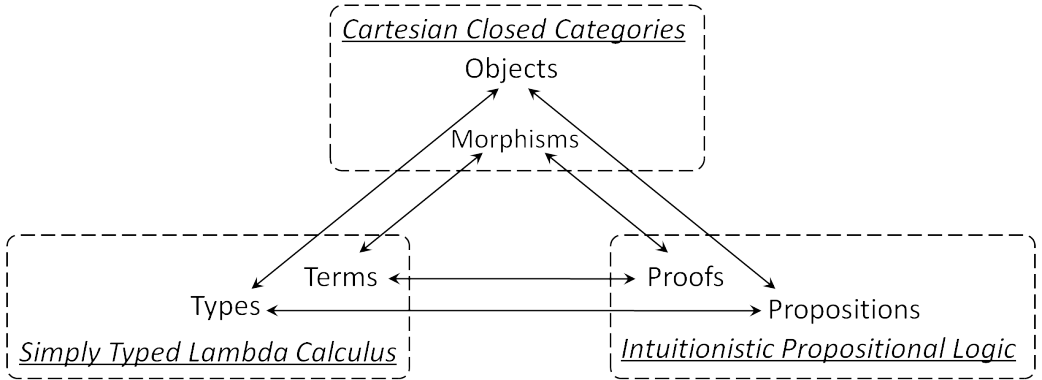
\includegraphics[width=0.9\textwidth]{./images/triangle}
\end{center}

Intuitionistic logic is a formalization of Brouwer’s intuitionism. As the founder of intuitionism, L. E. J. Brouwer avoided use of formal language or logic all his life. But his attitude did not stop others considering formalizations of parts of intuitionism. In the 1930s, Arend Heyting, a former student of Brouwer, produced the first complete axiomatizations for intuitionistic propositional and predicate logic. In intuitionistic logic, the law of excluded middle and double negation elimination are no longer axioms.

The lambda calculus was introduced by Alonzo Church in the early 1930s as a formal system to provide a functional foundation for mathematics. Since Church’s original system was shown to be logically inconsistent, he gave just a consistent subtheory of his original system dealing only with the functional part. Then, in 1940, Church also introduced a typed interpretation of the lambda calculus by giving each term a unique type. Today, the typed lambda calculus serves as the foundation of the modern type systems in computer science.

Category first appeared in Samuel Eilenberg and Saunders Mac Lane’s paper written in 1945. It was originally introduced to describe the passage from one type of mathematical structure to another. In recent decades, category theory has found use for computer science. For instant, it has a profound influence on the design of functional and imperative programming languages, e.g. Haskell and Agda.

Looking from the historical perspective, these three different systems seem to have different origins, not related to each other. However, Joachim Lambek showed in the early 1970s that cartesian closed categories provided a formal analogy between proofs in intuitionistic propositional logic and types in combinatory logic. As a result, some people may use Curry-Howard-Lambek Isomorphism to refer to this three-way-correspondence.

\newpage
\section{Background}
\include*{bg_il}
\include*{bg_lc}
\include*{bg_cat}

\newpage
\section{Correspondences}
\include*{co_t2p}
\include*{co_p2t}
\include*{co_t2m}


\newpage
\bibliographystyle{abbrv}
\bibliography{myref}
\nocite{*}
\addcontentsline{toc}{section}{References}

\end{document}
